\section{Элементы математической логики}

\subsection{Основные понятия}

\textbf{Математическая логика} -- это анализ методом рассуждений, при этом в первую очередь исследуются формы рассуждений, а не их содержание, т. е. математическая логика исследует соотношения между основными понятиями математики, на базе которых доказываются математические утверждения.

Простейшую из формальных логических теорий называют \textbf{алгеброй высказываний}.

\textbf{Высказыванием} называется утверждение (повествовательное предложение), о котором в данной ситуации можно сказать, что оно истинно или ложно, но не то и другое одновременно.

Высказыванию ставят в соответствие логическую переменную, которая принимает значение \(1\), если высказывание истинно, и \(0\), если высказывание ложно.

Из простых высказываний с помощью \textbf{логических связок} могут быть построены \textbf{составные высказывания}.

\subsection{Логические связки}

\subsubsection{Простейшие логические связки}

В таблице \ref{tab:simplest-logical-connectives} представлены простейшие логические связки.

{
\renewcommand*{\arraystretch}{1.5}
\begin{longtable}{|c|c|c|}
    \hline
    \textbf{Название} & \textbf{Прочтение}          & \textbf{Обозначение} \\
    \hline
    отрицание         & не                          & \(\lnot\)            \\
    \hline
    конъюнкция        & и                           & \(\land\)            \\
    \hline
    дизъюнкция        & или                         & \(\lor\)             \\
    \hline
    импликация        & если, то                    & \(\to\)              \\
    \hline
    эквивалентность   & тогда и только тогда, когда & \(\leftrightarrow\)  \\
    \hline
    \caption{Простейшие логические связки}
    \label{tab:simplest-logical-connectives}
\end{longtable}
}

Таблица \ref{tab:truth-table-slc} представляет собой таблицу истинности простейших логических связок.

{
\renewcommand*{\arraystretch}{1.5}
\begin{longtable}{|c|c|c|c|c|c|c|}
    \hline
    \(A\) & \(B\) & \(\bar{A}\) & \(A \land B\) & \(A \lor B\) & \(A \to B\) & \(A \leftrightarrow B\) \\
    \hline
    \(0\) & \(0\) & \(1\)       & \(0\)         & \(0\)        & \(1\)       & \(1\)                   \\
    \hline
    \(0\) & \(1\) & \(1\)       & \(0\)         & \(1\)        & \(1\)       & \(0\)                   \\
    \hline
    \(1\) & \(0\) & \(0\)       & \(0\)         & \(1\)        & \(0\)       & \(0\)                   \\
    \hline
    \(1\) & \(1\) & \(0\)       & \(1\)         & \(1\)        & \(1\)       & \(1\)                   \\
    \hline
    \caption{Таблица истинности простейших логических связок}
    \label{tab:truth-table-slc}
\end{longtable}
}


\subsubsection{Порядок выполнения логических операций}

Если скобок нет, то операции выполняются в следующем порядке:
\begin{enumerate}
    \item отрицание;
    \item конъюнкция;
    \item дизъюнкция;
    \item импликация;
    \item эквивалентность.
\end{enumerate}

\subsubsection{Доказательство тождественной истинности}

\begin{example*}
    Необходимо доказать тождественную истинность формулы
    \[
        \bar{A} \to (A \to B).
    \]

    {
    \renewcommand*{\arraystretch}{1.5}
    \begin{longtable}{|c|c|c|c|c|}
        \hline
        \(A\) & \(B\) & \(\bar{A}\) & \(A \to B\) & \(\bar{A} \to (A \to B)\) \\
        \hline
        \(0\) & \(0\) & \(1\)       & \(1\)       & \(1\)                     \\
        \hline
        \(0\) & \(1\) & \(1\)       & \(1\)       & \(1\)                     \\
        \hline
        \(1\) & \(0\) & \(0\)       & \(0\)       & \(1\)                     \\
        \hline
        \(1\) & \(1\) & \(0\)       & \(1\)       & \(1\)                     \\
        \hline
        \caption{Пример доказательства тождественной истинности}
    \end{longtable}
    }
\end{example*}

\subsubsection{Другие логические связки}

В таблице \ref{tab:other-logical-connectives} представлены другие логические связки, которые мы в дальнейшем будем использовать.

{
\renewcommand*{\arraystretch}{1.5}
\begin{longtable}{|c|c|c|}
    \hline
    \textbf{Название}   & \textbf{Прочтение}  & \textbf{Обозначение} \\
    \hline
    Штрих Шеффера       & антиконъюнкция      & \(|\)                \\
    \hline
    Стрелка Пирса       & антидизъюнкция      & \(\downarrow\)       \\
    \hline
    Сумма по модулю два & антиэквивалентность & \(\oplus\)           \\
    \hline
    \caption{Другие логические связки}
    \label{tab:other-logical-connectives}
\end{longtable}
}

Эти логические связки можно представить следующим образом:
\[
    A \mathop{|} B = \overline{A \land B};
    \quad
    A \downarrow B = \overline{A \lor B};
    \quad
    A \oplus B = \overline{A \leftrightarrow B}.
\]

Таблица \ref{tab:truth-table-olc} представляет собой таблицу истинности других логических связок.

{
\renewcommand*{\arraystretch}{1.5}
\begin{longtable}{|c|c|c|c|c|}
    \hline
    \(A\) & \(B\) & \(A \mathop{|} B\) & \(A \downarrow B\) & \(A \oplus B\) \\
    \hline
    \(0\) & \(0\) & \(1\)              & \(1\)              & \(0\)          \\
    \hline
    \(0\) & \(1\) & \(1\)              & \(0\)              & \(1\)          \\
    \hline
    \(1\) & \(0\) & \(1\)              & \(0\)              & \(1\)          \\
    \hline
    \(1\) & \(1\) & \(0\)              & \(0\)              & \(0\)          \\
    \hline
    \caption{Таблица истинности других логических связок}
    \label{tab:truth-table-olc}
\end{longtable}
}

\begin{note*}
    Таблицы истинности содержат \(2^n\) строк, где \(n\) -- число простых логических высказываний.
\end{note*}

\subsection{Логические отношения}

Отношение следствия: из \(A\) следует \(B\), если \(B\) истинно всякий раз, когда истинно \(A\).

\begin{example*}
    Рассмотрим высказывания \(A \leftrightarrow B\), \(A \to B\), \(A \lor B\):
    {
    \renewcommand*{\arraystretch}{1.5}
    \begin{longtable}{|c|c|c|c|c|}
        \hline
        \(A\) & \(B\) & \(A \leftrightarrow B\) & \(A \to B\) & \(A \lor B\) \\
        \hline
        \(0\) & \(0\) & \(1\)                   & \(1\)       & \(0\)        \\
        \hline
        \(0\) & \(1\) & \(0\)                   & \(1\)       & \(1\)        \\
        \hline
        \(1\) & \(0\) & \(0\)                   & \(0\)       & \(1\)        \\
        \hline
        \(1\) & \(1\) & \(1\)                   & \(1\)       & \(1\)        \\
        \hline
    \end{longtable}
    }
    Из \(A \leftrightarrow B\) следует \(A \to B\), однако из \(A \leftrightarrow B\) не следует \(A \lor B\).
\end{example*}

Два составных высказывания \textbf{эквивалентны}, если они имеют одинаковые истинностные значения на одинаковых наборах, т. е. последние столбцы их таблиц истинности должны совпадать.

\begin{example*}
    Проверим, являются ли высказывания \(A \to B\) и \(\bar{A} \lor B\) эквивалентными:

    \begin{minipage}[c]{0.5\textwidth}
        \renewcommand*{\arraystretch}{1.5}
        \begin{longtable}{|c|c|c|}
            \hline
            \(A\) & \(B\) & \(A \to B\) \\
            \hline
            \(0\) & \(0\) & \(1\)       \\
            \hline
            \(0\) & \(1\) & \(1\)       \\
            \hline
            \(1\) & \(0\) & \(0\)       \\
            \hline
            \(1\) & \(1\) & \(1\)       \\
            \hline
        \end{longtable}
    \end{minipage}
    \begin{minipage}[c]{0.5\textwidth}
        \renewcommand*{\arraystretch}{1.5}
        \begin{longtable}{|c|c|c|c|}
            \hline
            \(A\) & \(B\) & \(\bar{A}\) & \(\bar{A} \lor B\) \\
            \hline
            \(0\) & \(0\) & \(1\)       & \(1\)              \\
            \hline
            \(0\) & \(1\) & \(1\)       & \(1\)              \\
            \hline
            \(1\) & \(0\) & \(0\)       & \(0\)              \\
            \hline
            \(1\) & \(1\) & \(0\)       & \(1\)              \\
            \hline
        \end{longtable}
    \end{minipage}

    \vspace*{1em}

    Итого получим, что
    \[
        A \to B \equiv \bar{A} \lor B.
    \]
\end{example*}

\subsection{Варианты импликации}

\textbf{Импликация} двух высказываний отличается от эквивалентности, а также от дизъюнкции и конъюнкции тем, что она \textbf{несимметрична} (т. е. \(A \to B\) не эквивалентно \(B \to A\)).

Для высказывания \(A \to B\):
\begin{itemize}
    \item высказывание \(B \to A\) называется \textbf{конверсией};
    \item высказывание \(\bar{A} \to \bar{B}\) называется \textbf{конверсией контрапозиции};
    \item высказывание \(\bar{B} \to \bar{A}\) называется \textbf{контрапозицией}.
\end{itemize}

Таблица \ref{tab:truth-table-implication} представляет собой таблицу истинности этих вариантов импликации.

{
\renewcommand*{\arraystretch}{1.5}
\begin{longtable}{|c|c|c|c|c|c|c|c|}
    \hline
    \(A\) & \(B\) & \(\bar{A}\) & \(\bar{B}\) & \(A \to B\) & \(B \to A\) & \(\bar{A} \to \bar{B}\) & \(\bar{B} \to \bar{A}\) \\
    \hline
    \(0\) & \(0\) & \(1\)       & \(1\)       & \(1\)       & \(1\)       & \(1\)                   & \(1\)                   \\
    \hline
    \(0\) & \(1\) & \(1\)       & \(0\)       & \(1\)       & \(0\)       & \(0\)                   & \(1\)                   \\
    \hline
    \(1\) & \(0\) & \(0\)       & \(1\)       & \(0\)       & \(1\)       & \(1\)                   & \(0\)                   \\
    \hline
    \(1\) & \(1\) & \(0\)       & \(0\)       & \(1\)       & \(1\)       & \(1\)                   & \(1\)                   \\
    \hline
    \caption{Таблица истинности вариантов импликации}
    \label{tab:truth-table-implication}
\end{longtable}
}

\subsection{Необходимое и достаточное условия}

{
    \renewcommand*{\arraystretch}{1.5}
    \begin{longtable}{|C{0.27\textwidth}|C{0.27\textwidth}|C{0.27\textwidth}|}
        \hline
        \textbf{Условие}                                            & \textbf{Описание}                                               & \textbf{Операция}                                                 \\
        \hline
        \(A\) является достаточным условием для \(B\)               & Если имеет место \(A\), то \(B\) также будет иметь место        & Импликация \(A \to B\)                                            \\
        \hline
        \(A\) является необходимым условием для \(B\)               & Если имеет место \(B\), то \(A\) также будет иметь место        & Конверсия достаточного условия \(B \to A\)                        \\
        \hline
        \(A\) является необходимым и достаточным условием для \(B\) & \(A\) имеет место тогда и только тогда, когда имеет место \(B\) & Двойная импликация, т. е. эквивалентность \(A \leftrightarrow B\) \\
        \hline
    \end{longtable}
}

\subsection{Основные логические эквивалентности}

\begin{property}[Идемпотентность]
    \[
        A \lor A = A,
        \quad
        A \land A = A.
    \]
\end{property}

\begin{property}[Коммутативность]
    \[
        A \lor B = B \lor A,
        \quad
        A \land B = B \land A.
    \]
\end{property}

\begin{property}[Ассоциативность]
    \[
        A \lor (B \lor C) = (A \lor B) \lor C,
        \quad
        A \land (B \land C) = (A \land B) \land C.
    \]
\end{property}

\begin{property}[Дистрибутивность]
    \[
        A \lor (B \land C) = (A \lor B) \land (A \lor C),
        \quad
        A \land (B \lor C) = (A \land B) \lor (A \land C).
    \]
\end{property}

\begin{property}[Поглощение]
    \[
        (A \land B) \lor A = A,
        \quad
        (A \lor B) \land A = A.
    \]
\end{property}

\begin{property}[Свойства нуля]
    \[
        A \lor 0 = A,
        \quad
        A \land 0 = 0.
    \]
\end{property}

\begin{property}[Свойства единицы]
    \[
        A \lor 1 = 1,
        \quad
        A \land 1 = A.
    \]
\end{property}

\begin{property}[Инволютивность]
    \[
        \bar{\bar{A}} = A.
    \]
\end{property}

\begin{property}[Законы де Моргана]
    \[
        \overline{A \land B} = \bar{A} \lor \bar{B},
        \quad
        \overline{A \lor B} = \bar{A} \land \bar{B}.
    \]
\end{property}

\begin{property}[Свойства дополнения]
    \[
        A \lor \bar{A} = 1,
        \quad
        A \land \bar{A} = 0.
    \]
\end{property}

\begin{property}[Свойство импликации]
    \[
        A \to B = \bar{A} \lor B.
    \]
\end{property}

\begin{property}[Свойство эквивалентности]
    \[
        A \leftrightarrow B = (A \to B) \land (B \to A).
    \]
\end{property}

\subsection{Булевы функции}

\textbf{Булевы функции} находят применение в конструировании и упрощении логических схем.

Обозначим \(E_2 = \{0, 1\}\), тогда
\[
    E_2^n = \underbrace{E_2 \times E_2 \times \ldots \times E_2}_{n}.
\]

Функции \(f: E_2^n \to E_2\) называются \textbf{функции алгебры логики} или \textbf{булевыми функциями} от \(n\) переменных. Множество булевых функций от \(n\) переменных обозначают \(P_n\):
\[
    P_n = \{f \mid f : E_2^n \to E_2\}.
\]

\subsection{Множество булевых функций. Булев куб}

\(P_2\) -- множество всех булевых функций.

\(P_{2, n}\) -- множество всех булевых функций от \(n\) переменных:
\[
    P_{2, n} = \{f \mid f : E_2^n \to E_2\},
    \qquad
    P_2 = \bigcup_{n \geq 0} P_{2, n}.
\]

\(\{0, 1\}^n\) -- \textbf{булев куб} размерности \(n\). Число всех элементов булева куба \(\{0, 1\}^n\) составляет \(2^n\).

\subsection{Булев порядок}

Для произвольных наборов \(\bar{\alpha} = (\alpha_1, \ldots, \alpha_n)\) и \(\bar{\beta} = (\beta_1, \ldots, \beta_n)\) имеет место
\[
    \bar{\alpha} \leq \bar{\beta}
    \iff
    \alpha_i \leq \beta_i,
    \forall i = \overline{1, n}
\]
то есть
\[
    \bar{\alpha} \leq \bar{\beta}
    \iff
    \alpha_i = \beta_i
    \text{ или }
    \alpha_i, \beta_i = 1, \forall i = \overline{1, n}.
\]

Если существует хотя бы одно \(i\), для которого \(\alpha_i = 0\), \(\beta_i = 1\), то имеет место строгое неравенство \(\bar{\alpha} < \bar{\beta}\).

Если существует ровно одно \(i\), для которого \(\alpha_i = 0\), \(\beta_i = 1\), то набор \(\bar{\beta}\) \textbf{доминирует} над набором \(\bar{\alpha}\).

Рассмотренное отношение порядка на \(B^n\), где \(B^n\) -- \(n\)-я декартова степень
\[
    B = (\{0, 1\}, \lor, \land, 0, 1)
\]
будем называть \textbf{булевым порядком}.

Булев куб как упорядоченное множество можно изобразить в виде диаграммы Хассе
\begin{figure}[H]
    \centering
    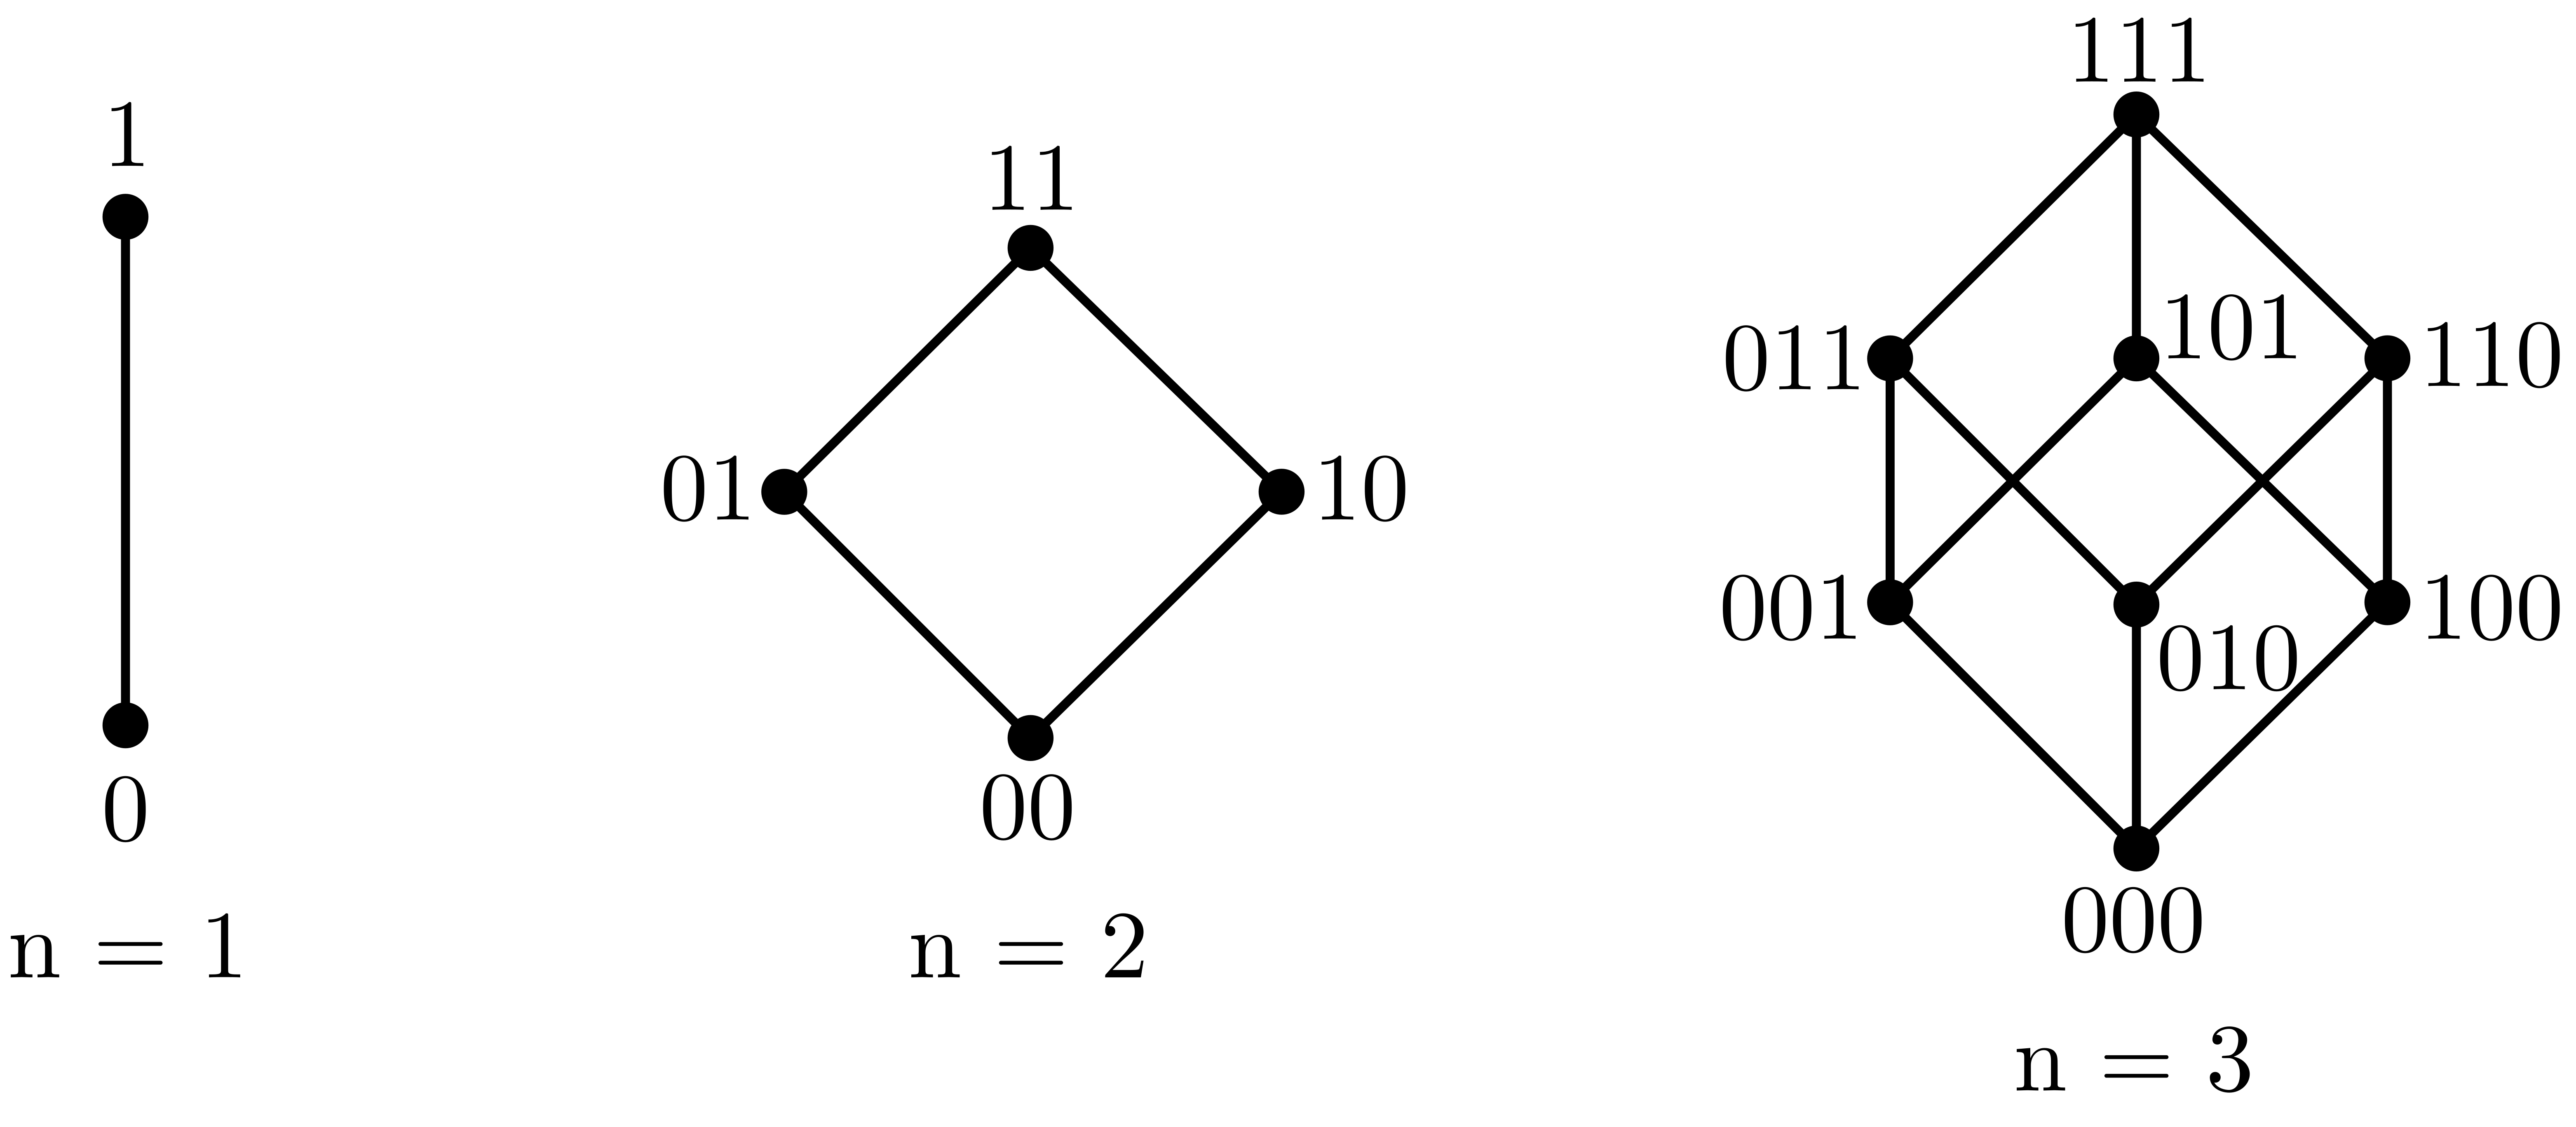
\includegraphics[width=0.9\textwidth]{images/boolean-cube.png}
    \caption{Примеры булевых кубов в виде диаграммы Хассе}
\end{figure}

\subsection{Мощность множества булевых функций}

\textbf{Число булевых функций} от \(n\) переменных находится по формуле
\[
    |P_{2, n}| = 2^{2^n}.
\]

{
\renewcommand*{\arraystretch}{1.5}
\begin{longtable}{|c|c|c|c|c|}
    \hline
    \(x_1\)    & \(\ldots\) & \(x_{n - 1}\) & \(x_n\)    & \(f(x_1, \ldots x_n)\) \\
    \hline
    \(0\)      & \(\ldots\) & \(0\)         & \(0\)      & \(f(0, \ldots, 0, 0)\) \\
    \hline
    \(0\)      & \(\ldots\) & \(0\)         & \(1\)      & \(f(0, \ldots, 0, 1)\) \\
    \hline
    \(0\)      & \(\ldots\) & \(1\)         & \(0\)      & \(f(0, \ldots, 1, 0)\) \\
    \hline
    \(\ldots\) & \(\ldots\) & \(\ldots\)    & \(\ldots\) & \(\ldots\)             \\
    \hline
    \(1\)      & \(\ldots\) & \(1\)         & \(1\)      & \(f(1, \ldots, 1, 1)\) \\
    \hline
    \caption{Таблица булевых функций}
\end{longtable}
}

\subsection{Существенные и несущественные переменные}

Булева функция \(f \in P_n\) \textbf{существенно зависит} от переменной \(x_i\), если существует такой набор значений
\[
    a_1, \ldots, a_{i - 1}, a_{i +1}, \ldots, a_n
\]

что
\[
    f(a_1, \ldots, a_{i - 1}, 0, a_{i +1}, \ldots, a_n) \neq f(a_1, \ldots, a_{i - 1}, 0, a_{i +1}, \ldots, a_n).
\]

В этом случае \(x_i\) называют \textbf{существенной} переменной, в противном случае \(x_i\) называют \textbf{несущественной} (фиктивной) переменной.

\begin{example*}
    Рассмотрим следующую таблицу истинности:

    \vspace*{1em}

    {
        \renewcommand*{\arraystretch}{1.5}
        \begin{longtable}{|c|c|c|c|}
            \hline
            \(x_1\) & \(x_2\) & \(f_1\) & \(f_2\) \\
            \hline
            \(0\)   & \(0\)   & \(0\)   & \(1\)   \\
            \hline
            \(0\)   & \(1\)   & \(0\)   & \(1\)   \\
            \hline
            \(1\)   & \(0\)   & \(1\)   & \(0\)   \\
            \hline
            \(1\)   & \(1\)   & \(1\)   & \(0\)   \\
            \hline
        \end{longtable}
    }

    В данном случае \(x_1\) -- существенная переменная, а \(x_2\) -- несущественная, поскольку
    \begin{gather*}
        f_1(0, 0) = f_1(0, 1),
        \quad
        f_1(1, 0) = f_1(1, 1).
        \\
        f_2(0, 0) = f_2(0, 1),
        \quad
        f_2(1, 0) = f_2(1, 1).
    \end{gather*}
\end{example*}

\subsection{Булевы функции одной и нескольких переменной}

{
    \renewcommand*{\arraystretch}{1.5}
    \begin{longtable}{|c|c|c|c|c|}
        \hline
        \(x\) & \(f_1\) & \(f_2\) & \(f_3\) & \(f_4\) \\
        \hline
        \(0\) & \(0\)   & \(0\)   & \(1\)   & \(1\)   \\
        \hline
        \(1\) & \(0\)   & \(1\)   & \(0\)   & \(1\)   \\
        \hline
        \caption{Булевы функции одной переменной}
    \end{longtable}
}

{
    \setlength{\tabcolsep}{3pt}
    \renewcommand*{\arraystretch}{1.5}
    \begin{longtable}{|c|c!{\vrule width 1.2pt}Sc|c|c|c|c|c|c|c|c|c|c|c|c|c|c|c|c|}
        \hline
        \(x_1\) & \(x_2\) & \(f_1\) & \(f_2\) & \(f_3\) & \(f_4\) & \(f_5\) & \(f_6\) & \(f_7\) & \(f_8\) & \(f_9\) & \(f_{10}\) & \(f_{11}\) & \(f_{12}\) & \(f_{13}\) & \(f_{14}\) & \(f_{15}\) & \(f_{16}\) \\
        \hline
        \(0\)   & \(0\)   & \(0\)   & \(0\)   & \(0\)   & \(0\)   & \(0\)   & \(0\)   & \(0\)   & \(0\)   & \(1\)   & \(1\)      & \(1\)      & \(1\)      & \(1\)      & \(1\)      & \(1\)      & \(1\)      \\
        \hline
        \(0\)   & \(1\)   & \(0\)   & \(0\)   & \(0\)   & \(0\)   & \(1\)   & \(1\)   & \(1\)   & \(1\)   & \(0\)   & \(0\)      & \(0\)      & \(0\)      & \(1\)      & \(1\)      & \(1\)      & \(1\)      \\
        \hline
        \(1\)   & \(0\)   & \(0\)   & \(0\)   & \(1\)   & \(1\)   & \(0\)   & \(0\)   & \(1\)   & \(1\)   & \(0\)   & \(0\)      & \(1\)      & \(1\)      & \(0\)      & \(0\)      & \(1\)      & \(1\)      \\
        \hline
        \(1\)   & \(1\)   & \(0\)   & \(1\)   & \(0\)   & \(1\)   & \(0\)   & \(1\)   & \(0\)   & \(1\)   & \(0\)   & \(1\)      & \(0\)      & \(1\)      & \(0\)      & \(1\)      & \(0\)      & \(1\)      \\
        \hline
        \caption{Булевы функции двух переменных}
    \end{longtable}
}

\subsection{Мажоритарная функция}

{
    \renewcommand*{\arraystretch}{1.5}
    \begin{longtable}{|c|c|c|c|c|}
        \hline
              & \(x_1\) & \(x_2\) & \(x_3\) & \(f(x_1, x_2, x_3)\) \\
        \hline
        \(0\) & \(0\)   & \(0\)   & \(0\)   & \(0\)                \\
        \hline
        \(1\) & \(0\)   & \(0\)   & \(1\)   & \(0\)                \\
        \hline
        \(2\) & \(0\)   & \(1\)   & \(0\)   & \(0\)                \\
        \hline
        \(3\) & \(0\)   & \(1\)   & \(1\)   & \(1\)                \\
        \hline
        \(4\) & \(1\)   & \(0\)   & \(0\)   & \(0\)                \\
        \hline
        \(5\) & \(1\)   & \(0\)   & \(1\)   & \(1\)                \\
        \hline
        \(6\) & \(1\)   & \(1\)   & \(0\)   & \(1\)                \\
        \hline
        \(7\) & \(1\)   & \(1\)   & \(1\)   & \(1\)                \\
        \hline
        \caption{Мажоритарная функция (функция голосования)}
    \end{longtable}
}

\subsection{Реализация функций формулами}

Так же, как составные высказывания строятся из более простых, с помощью логических операций, можно комбинировать булевы переменные с помощью булевых операций, получая булевы выражения, которые называются \textbf{формулами}. Всякой формуле однозначно соответствует некоторая функция, при этом говорят, что \textbf{формула реализует функцию}.

\begin{example*}
    Построим таблицу истинности для формулы
    \[
        ((x_1 \land x_2) \oplus x_1) \oplus x_2.
    \]

    {
    \renewcommand*{\arraystretch}{1.5}
    \begin{longtable}{|c|c|c|c|c|}
        \hline
        \(x_1\) & \(x_2\) & \(x_1 \land x_2\) & \((x_1 \land x_2) \oplus x_1\) & \(((x_1 \land x_2) \oplus x_1) \oplus x_2\) \\
        \hline
        \(0\)   & \(0\)   & \(0\)             & \(0\)                          & \(0\)                                       \\
        \hline
        \(0\)   & \(1\)   & \(0\)             & \(0\)                          & \(1\)                                       \\
        \hline
        \(1\)   & \(0\)   & \(0\)             & \(1\)                          & \(1\)                                       \\
        \hline
        \(1\)   & \(1\)   & \(1\)             & \(0\)                          & \(1\)                                       \\
        \hline
    \end{longtable}
    }

    Формула \(((x_1 \land x_2) \oplus x_1) \oplus x_2\) реализует функцию \(f_8(x_1, x_2) = 0111\).
\end{example*}

\subsection{Равносильные формулы}

Одна функция может иметь множество реализацией. Формулы, реализующие одну и ту же функцию, называются \textbf{равносильными}:
\[
    \mathcal{F}_1 = \mathcal{F}_2
    \iff
    \exists f: \text{func} \; \mathcal{F}_1 = f \land \text{func} \; \mathcal{F}_2 = f.
\]

Другими словами, булевы функции \(f\) и \(g\) называют равносильными, если их существенные переменные соответственно равны и на каждом наборе значений этих переменных функции \(f\) и \(g\) принимают равные значения.

\begin{example*}
    Пусть
    \[
        f(x, y) = x \lor y,
        \quad
        g(x, y, z) = xz \lor x \bar{z} \lor yz \lor y \bar{z}.
    \]

    Упростим функцию \(g(x, y, z)\):
    \[
        g(x, y, z) =
        xz \lor x \bar{z} \lor yz \lor y \bar{z} =
        x(z \lor \bar{z}) \lor y(z \lor \bar{z}) =
        x \lor y.
    \]

    Получили, что функции \(f(x, y)\) и \(g(x, y, z)\) равносильны.
\end{example*}

\subsection{Законы булевой алгебры}

\begin{property}[Идемпотентность]
    \[
        a \lor a = a,
        \quad
        a \land a = a.
    \]
\end{property}

\begin{property}[Коммутативность]
    \[
        a \lor b = b \lor a,
        \quad
        a \land b = b \land a.
    \]
\end{property}

\begin{property}[Ассоциативность]
    \[
        a \lor (b \lor c) = (a \lor b) \lor c,
        \quad
        a \land (b \land c) = (a \land b) \land c.
    \]
\end{property}

\begin{property}[Дистрибутивность]
    \[
        a \lor (b \land c) = (a \lor b) \land (a \lor c),
        \quad
        a \land (b \lor c) = (a \land b) \lor (a \land c).
    \]
\end{property}

\begin{property}[Поглощение]
    \[
        (a \land b) \lor a = a,
        \quad
        (a \lor b) \land a = a.
    \]
\end{property}

\begin{property}[Свойства нуля]
    \[
        a \lor 0 = a,
        \quad
        a \land 0 = 0.
    \]
\end{property}

\begin{property}[Свойства единицы]
    \[
        a \lor 1 = 1,
        \quad
        a \land 1 = a.
    \]
\end{property}

\begin{property}[Инволютивность]
    \[
        \bar{\bar{a}} = a.
    \]
\end{property}

\begin{property}[Законы де Моргана]
    \[
        \overline{a \land b} = \bar{a} \lor \bar{b},
        \quad
        \overline{a \lor b} = \bar{a} \land \bar{b}.
    \]
\end{property}

\begin{property}[Свойства дополнения]
    \[
        a \lor \bar{a} = 1,
        \quad
        a \land \bar{a} = 0.
    \]
\end{property}

\begin{property}[Свойство импликации]
    \[
        a \to b = \bar{a} \lor b.
    \]
\end{property}

\begin{property}[Свойство эквивалентности]
    \[
        a \leftrightarrow b = (a \to b) \land (b \to a).
    \]
\end{property}

\subsection{Двойственная функция}

Пусть \(f(x_1, \ldots, x_n) \in P_n\) -- булева функция. Тогда функция
\[
    f^*(x_1, \ldots, x_n) = \overline{f(\bar{x}_1, \ldots, \bar{x}_n)}
\]
называется \textbf{двойственной} к функции \(f\).

\begin{example}
    \[
        0^* = \bar{0} = 1.
    \]
\end{example}

\begin{example}
    \[
        1^* = \bar{1} = 0.
    \]
\end{example}

\begin{example}
    \[
        x^* = \bar{\bar{x}} = x.
    \]

    Т. к. \(x\) в данном случае и функция, и переменная, мы применяем двойное отрицание.
\end{example}

\begin{example}
    \[
        (x \land y)^* = \overline{\bar{x} \land \bar{y}} = x \lor y.
    \]
\end{example}

\begin{example}
    \[
        (x \lor y)^* = \overline{\bar{x} \lor \bar{y}} = x \land y.
    \]
\end{example}

\subsection{Инволютивность двойственности}

Из определения видно, что двойственность инволютивна: \(f^{**} = f\), поэтому отношение <<быть двойственной к>> на множестве булевых функций симметрично, то есть, если \(f^* = g\), то \(g^* = f\).

Если в таблице истинности булевой функции \(f\) инвертировать все значения, то получим таблицу истинности двойственной функции \(f^*\).

\subsection{Самодвойственная функция}

Функция называется \textbf{самодвойственной}, если \(f^* = f\). Примером такой функции может служить функция \(f(x) = x\):
\[
    x^* = \bar{\bar{x}} = x.
\]

\subsection{Принцип двойственности}

\begin{theorem*}
    Пусть \(F = \{f_1, \ldots, f_m\}\) -- система булевых функций, а \(F^* = \{f_1^*, \ldots, f_n^*\}\) -- система двойственных функций. Тогда если формула \(\mathcal{F}\) над базисом \(F\) реализует функцию \(f\), то формула \(\mathcal{F}^*\) над базисом \(F^*\), полученная заменой функций \(f_i\), двойственными функциями \(f_i^*\), реализует функцию \(f^*\):
    \[
        \text{func} \; \mathcal{F} |F| = f
        \implies
        \text{func} \; \mathcal{F}^* |F^*| = f^*.
    \]

    \begin{consequence*}
        Если две равносильные формулы заменить двойственными, то равносильность сохранится:
        \[
            \mathcal{F}_1 = \mathcal{F}_2
            \implies
            \mathcal{F}_1^* = \mathcal{F}_2^*.
        \]
    \end{consequence*}
\end{theorem*}

\begin{note*}
    Формула, двойственная к булевой формуле, может быть получена заменой констант \(0\) на \(1\), \(1\) на \(0\), операций \(\land\) на \(\lor\), \(\lor\) на \(\land\) и сохранением структуры формулы.
\end{note*}

\subsection{Нормальные формы}

Если \(x\) -- логическая переменная, \(\sigma \in \{0, 1\}\), то выражение
\[
    x^\sigma =
    \begin{dcases}
        x, \text{если } \sigma = 1, \\
        \bar{x}, \text{если } \sigma = 0.
    \end{dcases}
\]
называется литерой. Литеры \(x\) и \(\bar{x}\) называются \textbf{контрарными}. \textbf{Элементарной конъюнкцией} называется конъюнкция литер. \textbf{Элементарной дизъюнкцией} называется дизъюнкция литер.

\subsection{ДНФ и КНФ}

Дизъюнкция элементарных конъюнкций называется \textbf{дизъюнктивной нормальной формой (ДНФ)}.

Конъюнкция элементарных дизъюнкций называется \textbf{конъюнктивной нормальной формой (КНФ)}.

\begin{example}
    ДНФ:
    \[
        (x \land \bar{y}) \lor (y \land z).
    \]
\end{example}

\begin{example}
    КНФ:
    \[
        (x \lor z \lor \bar{y}) \land (x \lor y) \land z.
    \]
\end{example}

\begin{example}
    Одновременно и КНФ, и ДНФ:
    \[
        x \land \bar{y}.
    \]
\end{example}

\begin{theorem*}
    \newpar
    \begin{enumerate}
        \item Любая формула эквивалентна некоторой ДНФ.
        \item Любая формула эквивалентна некоторой КНФ.
    \end{enumerate}
\end{theorem*}

\noindent \textbf{Алгоритм приведения формулы к ДНФ:}
\begin{enumerate}
    \item выразить все логические операции, участвующие в построении формулы, через дизъюнкцию, конъюнкцию и отрицание;
    \item используя законы де Моргана, перенести все отрицания к переменным;
    \item убрать двойные отрицания;
    \item используя закон дистрибутивности, преобразовать формулу так, чтобы все конъюнкции выполнялись раньше дизъюнкций.
\end{enumerate}

\noindent \textbf{Алгоритм приведения формулы к КНФ:}
\begin{enumerate}
    \item выразить все логические операции, участвующие в построении формулы, через дизъюнкцию, конъюнкцию и отрицание;
    \item используя законы де Моргана, перенести все отрицания к переменным;
    \item убрать двойные отрицания;
    \item используя закон дистрибутивности, преобразовать формулу так, чтобы все дизъюнкции выполнялись раньше, чем конъюнкции.
\end{enumerate}

\subsection{Совершенные нормальные формы}

\subsubsection{СДНФ}

Реализация булевой функции \(f(x_1, \ldots, x_n)\) в виде формулы
\[
    f(x_1, \ldots, x_n) = \biglor x_1^{\sigma_1} \land \ldots \land x_n^{\sigma_n}
\]
называется \textbf{совершенной дизъюнктивной нормальной формой (СДНФ)}. Таким образом, СДНФ есть ДНФ, в которой нет одинаковых элементарных конъюнкций, и в каждой элементарной конъюнкции каждая переменная \(x_i\), из набора \(\{x_1, \ldots, x_n\}\) входит ровно один раз, причем входит либо сама \(x_i\), либо ее отрицание \(\bar{x}_i\).

\begin{theorem*}
    Каждая булева функция, отличная от константы \(0\), имеет единственную СДНФ.
\end{theorem*}

\subsubsection{СКНФ}

Реализация булевой функции \(f(x_1, \ldots, x_n)\) в виде формулы
\[
    f(x_1, \ldots, x_n) = \bigland x_1^{\sigma_1} \lor \ldots \lor x_n^{\sigma_n}
\]
называется \textbf{совершенной конъюнктивной нормальной формой (СКНФ)}. Таким образом, СКНФ есть КНФ, в которой нет одинаковых элементарных дизъюнкций, и в каждой элементарной дизъюнкции каждая переменная \(x_i\) из набора \(\{x_1, \ldots, x_n\}\) входит ровно один раз, причем входит либо сама \(x_i\), либо ее отрицание \(\bar{x}_i\).

\begin{theorem*}
    Всякая булева функция, отличная от константы \(1\), имеет единственную СКНФ.
\end{theorem*}

\subsection{Нахождение СДНФ}

\noindent При нахождении СДНФ пользуются следующим правилом:
\begin{enumerate}
    \item каждый набор аргументов определяет элементарную конъюнкцию, в которой значению \(0\) соответствует отрицание переменной, а значению \(1\) -- сама переменная.
    \item СДНФ функции образуют те элементарные конъюнкции, которые соответствуют наборам аргументов, дающим \(1\).
\end{enumerate}

Каждый набор аргументов, на котором функция принимает значение \(1\), называется \textbf{конституентой единицы} функции.

\begin{example*}
    Найдем СДНФ для \(x_1 \to x_2\).

        {
            \renewcommand{\arraystretch}{1.5}
            \begin{longtable}{|c|c|c|c|}
                \hline
                \(x_1\) & \(x_2\) & \(x_1 \to x_2\) & элем. конъюнкции              \\
                \hline
                \(0\)   & \(0\)   & \(1\)           & \(\bar{x}_1 \land \bar{x}_2\) \\
                \hline
                \(0\)   & \(1\)   & \(1\)           & \(\bar{x}_1 \land x_2\)       \\
                \hline
                \(1\)   & \(0\)   & \(0\)           & \(x_1 \land \bar{x}_2\)       \\
                \hline
                \(1\)   & \(1\)   & \(1\)           & \(x_1 \land x_2\)             \\
                \hline
            \end{longtable}
        }

    СДНФ: \((\bar{x}_1 \land \bar{x}_2) \lor (\bar{x}_1 \land x_2) \lor (x_1 \land x_2)\).
\end{example*}

\subsection{Нахождение СКНФ}

\noindent При нахождении СКНФ пользуются следующим правилом:
\begin{enumerate}
    \item каждый набор аргументов определяет элементарную дизъюнкцию, в которой значению \(1\) соответствует инверсия переменной, а значению \(0\) -- сама переменная;
    \item СКНФ функции образуют те элементарные конъюнкции, которые соответствуют наборам аргументов, дающим \(0\).
\end{enumerate}

Каждый набор аргументов, на котором функция принимает значение \(0\), называется \textbf{конституентой нуля} функции.

\begin{example}
    Найдем СКНФ для \(x_1 \to x_2\).

        {
            \renewcommand{\arraystretch}{1.5}
            \begin{longtable}{|c|c|c|c|}
                \hline
                \(x_1\) & \(x_2\) & \(x_1 \to x_2\) & элем. дизъюнкции             \\
                \hline
                \(0\)   & \(0\)   & \(1\)           & \(x_1 \lor x_2\)             \\
                \hline
                \(0\)   & \(1\)   & \(1\)           & \(x_1 \lor \bar{x}_2\)       \\
                \hline
                \(1\)   & \(0\)   & \(0\)           & \(\bar{x}_1 \lor x_2\)       \\
                \hline
                \(1\)   & \(1\)   & \(1\)           & \(\bar{x}_1 \lor \bar{x}_2\) \\
                \hline
            \end{longtable}
        }

    СКНФ: \(\bar{x}_1 \lor x_2\).
\end{example}

\subsection{Замкнутые классы}

Пусть
\[
    F = \{f_1, \ldots, f_m\}, f_i \in P_2 \; \forall i \in \overline{1, m}.
\]

Замыканием \(F\) называется множество всех булевых функций, реализуемых формулами над \(F\):
\[
    [F] = \{f \in P_2 \mid f = \text{func} \; F [F]\}.
\]

Класс функций, сохраняющих \(0\):
\[
    T_0 = \{f \in P_2 \mid f(0, \ldots, 0) = 0\}.
\]

Класс функций, сохраняющих \(1\):
\[
    T_1 = \{f \in P_2 \mid f(1, \ldots, 1) = 1\}.
\]

Класс самодвойственных функций:
\[
    S = \{f \in P_2 \mid f = f^*\}.
\]

Класс монотонных функций:
\[
    M = \{f \in P_2 \mid \forall \alpha, \beta : \alpha \leq \beta \implies f(\alpha) \leq f(\beta)\}.
\]

Класс линейных функций:
\[
    L = \{f \in P_2 \mid f(x_1, \ldots, x_n) = a_0 \oplus a_1 x_1 \oplus \ldots \oplus a_n x_n\}.
\]

\begin{theorem*}
    Классы \(T_0\), \(T_1\), \(S\), \(M\), \(L\) -- замкнуты.
\end{theorem*}

\begin{example*}
    Рассмотрим конъюнкцию и введем обозначение \(\psi(x, y) = x \land y\). Построим таблицу истинности:
    {
    \renewcommand*{\arraystretch}{1.5}
    \begin{longtable}{|c|c|c|c|}
        \hline
        \(x\) & \(y\) & \(\psi(x, y) = x \land y\) & треугольник \\
        \hline
        \(0\) & \(0\) & \(0\)                      & \(0001\)    \\
        \hline
        \(0\) & \(1\) & \(0\)                      & \(001\)     \\
        \hline
        \(1\) & \(0\) & \(0\)                      & \(01\)      \\
        \hline
        \(1\) & \(1\) & \(1\)                      & \(1\)       \\
        \hline
    \end{longtable}
    }
    Тогда:
    \begin{itemize}
        \item \(\psi \in T_0\), т. к. \(0 \land 0 = 0\);
        \item \(\psi \in T_1\), т. к. \(1 \land 1 = 1\);
        \item \(\psi \notin S\), т. к. \(\psi^*(x, y) = \overline{\bar{x} \land \bar{y}} = x \lor y \neq \psi(x, y)\);
        \item \(\psi \in M\), можно убедиться, посмотрев на таблицу истинности;
        \item \(\psi \notin L\), можно убедиться, построив полином Жегалкина:
              \[
                  \psi(x, y) = xyz.
              \]
    \end{itemize}
\end{example*}

\subsection{Свойства замыкания}

\begin{property}
    \[
        F \subset [F]
    \]
\end{property}

\begin{property}[Идемпотентность]
    \[
        [[F]] = [F]
    \]
\end{property}

\begin{property}[Монотонность]
    \[
        F_1 \subset F_2 \implies [F_1] \subset [F_2]
    \]
\end{property}

\begin{property}
    \[
        ([F_1] \cup [F_2]) \subset [F_1 \cup F_2].
    \]
\end{property}

Класс (множество) функций \(F\) называется \textbf{замкнутым}, если \([F] = F\).

\subsection{Полные системы функций}

Класс функций \(F\) называется \textbf{полным}, если его замыкание совпадает с \(P_2\):
\[
    [F] = P_2.
\]

Другими словами, множество функции \(F\) образует полную систему, если любая булева функция реализуема в виде формулы над \(F\).

\begin{theorem*}
    Пусть заданы две системы функций
    \[
        F = \{f_1, \ldots, f_m\},
        \quad
        G = \{g_1, \ldots, g_k\}
    \]
    Тогда, если система \(F\) полна и все функции из \(F\) реализуемы формулами над \(G\), то система \(G\) также полна.
\end{theorem*}

\begin{example*}
    Система \(\{\lor, \land, \neg\}\) полная, т. к. всякая булева функция (в силу того, что она имеет единственную СДНФ) может быть выражена через дизъюнкцию, конъюнкцию и отрицание. Тогда
    \begin{itemize}
        \item система \(\{\neg, \land\}\) полная, т. к.
              \[
                  x_1 \lor x_2 = \overline{\bar{x}_1 \land \bar{x}_2};
              \]
        \item система \(\{\neg, \lor\}\) полная, т. к.
              \[
                  x_1 \land x_2 = \overline{\bar{x}_1 \lor \bar{x}_2};
              \]
        \item система \(\{\mid\}\) полная, т. к.
              \[
                  \bar{x} = x \mid x,
                  \quad
                  x_1 \land x_2 = \overline{x_1 \mid x_2} = (x_1 \mid x_2) \mid (x_1 \mid x_2);
              \]
        \item система \(\{0, 1, \land, \oplus\}\) полная, т. к.
              \[
                  \bar{x} = x \oplus 1.
              \]
    \end{itemize}
\end{example*}

\subsection{Полнота двойственной системы}

\begin{theorem*}
    Если система \(F = \{f_1, \ldots, f_m\}\) полна, то система \(F^* = \{f_1^*, \ldots, f_m^*\}\) также полна.
\end{theorem*}

\begin{example*}
    Система \(\{0, 1, \land, \oplus\}\) полна, следовательно, система \(\{1, 0, \lor, \leftrightarrow\}\) также полна.
\end{example*}

\subsection{Теорема Поста}

\begin{theorem*}
    Система булевых функций \(F\) полна тогда и только тогда, когда она содержит:
    \begin{itemize}
        \item хотя бы одну функцию, не сохраняющую ноль;
        \item хотя бы одну функцию, не сохраняющую единицу;
        \item хотя бы одну несамодвойственную функцию;
        \item хотя бы одну немонотонную функцию;
        \item хотя бы одну нелинейную функцию.
    \end{itemize}

    \[
        [F] = P_2
        \iff
        \overline{F \subset T_0 \lor F \subset T_1 \lor F \subset S \lor F \subset M \lor F \subset L}.
    \]
\end{theorem*}

\begin{example}
    Рассмотрим систему \(\{\lor, \land, \neg\}\):
    {
    \renewcommand*{\arraystretch}{1.5}
    \begin{longtable}{|c|c|c|c|c|c|}
        \hline
                          & \(T_0\) & \(T_1\) & \(S\) & \(M\) & \(L\) \\
        \hline
        \(\bar{x}\)       & \(-\)   & \(-\)   & \(+\) & \(-\) & \(+\) \\
        \hline
        \(x_1 \land x_2\) & \(+\)   & \(+\)   & \(-\) & \(+\) & \(-\) \\
        \hline
        \(x_1 \lor x_2\)  & \(+\)   & \(+\)   & \(-\) & \(+\) & \(-\) \\
        \hline
    \end{longtable}
    }
    Так как в каждом столбике есть \(-\), система \(\{\lor, \land, \neg\}\) -- полная. Также очевидно, что \(\{\land, \neg\}\) и \(\{\lor, \neg\}\) являются полными, а значит являются базисами для исходной системы.
\end{example}

\begin{example}
    Рассмотрим систему \(\{\mid\}\):
    {
    \renewcommand*{\arraystretch}{1.5}
    \begin{longtable}{|c|c|c|c|}
        \hline
        \(x\) & \(y\) & \(f(x, y) = x \mid y\) & треугольник \\
        \hline
        \(0\) & \(0\) & \(1\)                  & \(1110\)    \\
        \hline
        \(0\) & \(1\) & \(1\)                  & \(001\)     \\
        \hline
        \(1\) & \(0\) & \(1\)                  & \(01\)      \\
        \hline
        \(1\) & \(1\) & \(0\)                  & \(1\)       \\
        \hline
    \end{longtable}
    }

    \begin{enumerate}
        \item \(f(0, 0) = 1 \implies f \notin T_0\);
        \item \(f(1, 1) = 0 \implies f \notin T_1\);
        \item \(f(0, 1) = 1, f(1, 0) = 1 \implies f \notin S\);
        \item \((0, 0) < (1, 1), f(0, 0) > f(1, 1) \implies f \notin M\);
        \item \(f(x, y) = 1 \oplus xy \implies f \notin L\).
    \end{enumerate}

    {
    \renewcommand*{\arraystretch}{1.5}
    \begin{longtable}{|c|c|c|c|c|c|}
        \hline
                     & \(T_0\) & \(T_1\) & \(S\) & \(M\) & \(L\) \\
        \hline
        \(x \mid y\) & \(-\)   & \(-\)   & \(-\) & \(-\) & \(-\) \\
        \hline
    \end{longtable}
    }

    Следовательно, система \(\{|\}\) является полной по критерию Поста. Таким же образом можно доказать, что \({\downarrow}\) также является полной.
\end{example}

\begin{note*}
    Число шефферовых функций от \(n\) переменных равно
    \[
        2^{2^n - 2} - 2^{2^{n - 1} - 1}.
    \]
\end{note*}

\subsection{Одноместный предикат}

\textbf{Одноместный предикат} \(P(x)\) -- это функция переменной \(x\), определенная на множестве \(M\) и принимающая значения на множестве \(\{0, 1\}\). Те значения переменной, на которых предикат принимает истинное значение, образуют \textbf{множество истинности предиката}. Так как предикаты принимают значения \(0\) и \(1\), то к ним применяются логические операции.

\begin{example*}
    Пусть даны предикаты \(P(x) = \text{<<\(x\) -- четное число>>}\) и \(Q(x) = \text{<<\(x\) кратно \(3\)>>}\), определенные на множестве \(M = \{1, 2, 3, 4, 5, 6, 7, 8, 9\}\). Необходимо найти область истинности предикатов:
    \begin{enumerate}
        \item \(P(x) \land Q(x)\);
        \item \(P(x) \lor Q(x)\);
        \item  \(\bar{P}(x)\);
        \item \(P(x) \to Q(x)\).
    \end{enumerate}
    Решение:
    \begin{enumerate}
        \item \(I_{P \land Q} = I_P \cap I_Q = \{6\}\);
        \item \(I_{P \lor Q} = I_P \cup I_Q = \{2, 3, 4, 6, 8 ,9\}\);
        \item \(I_{\bar{P}} = \bar{I}_P = M \setminus I_P = \{1, 3, 5, 7, 9\}\);
        \item \(I_{P \to Q} = \bar{I}_P \cup I_Q = \{1, 3, 5, 6, 7, 9\}\).
    \end{enumerate}
\end{example*}

\subsection{n-местный предикат}

\(n\)-местным предикатом называется функция \(n\) переменных \(P(x_1, \ldots, x_n)\), определенная на множестве \(M = M_1 \times \ldots \times M_n\) и принимающая на этом множестве одно из двух значений: истина или ложь:
\[
    P(x_1, \ldots, x_n) : M_1 \times \ldots \times M_n \to E_2.
\]

\subsection{Кванторные операции}

Пусть \(P(x)\) -- одноместный предикат, определенный на множестве \(M\). Квантор общности \(\forall\) превращает предикат \(P(x)\) в высказывание:
\[
    \forall P(x) = \text{<<для любого элемента \(x\) высказывание \(P(x)\) истинно>>}.
\]

Квантор существования \(\exists\) превращает предикат \(P(x)\) в высказывание
\[
    \exists P(x) = \text{<<существует элемент \(x\) такой, что высказывание \(P(x)\) истинно>>}.
\]

Операция приписывания к предикату квантора называется \textbf{навешиванием квантора}. Переменная, к которой относится квантор, связывается квантором и называется \textbf{связанной переменной}. Переменная, не связанная квантором, называется \textbf{свободной переменной}.

\subsection{Алфавит логики предикатов}

\begin{enumerate}
    \item предметные константы \(p\), \(q\), \(r\), \(\ldots\) (принимают значения \(0\) или \(1\));
    \item предметные переменные \(x\), \(y\), \(z\), \(\ldots\), пробегающие значения некоторого множества \(M\);
    \item функциональные переменные \(f\), \(g\), \(h\), \(\ldots\);
    \item предикатные переменные \(P\), \(Q\), \(R\), \(\ldots\);
    \item символы логических операций \(\land\), \(\lor\), \(\to\), \(\neg\);
    \item кванторные символы \(\forall\), \(\exists\);
    \item запятая, скобки.
\end{enumerate}

\subsection{Формулы логики предикатов}

\noindent Определим понятие \textbf{терма}:
\begin{enumerate}
    \item Всякая предметная константа есть терм.
    \item Всякая предметная переменная есть терм.
    \item Если \(t_1, \ldots, t_n\) -- термы, а \(f\) -- функциональная переменная, то \(f(t_1, \ldots, t_n)\) -- есть терм.
\end{enumerate}

\noindent Определим понятие \textbf{формулы}:
\begin{enumerate}
    \item Если \(t_1, \ldots, t_n\) -- термы, \(\{x_1, \ldots, x_n\}\) -- множество всех переменных в термах \(t_1, \ldots, t_n\), \(P\) -- предикатная переменная, то \(P(t_1, \ldots, t_n)\) -- элементарная формула со свободными переменными \(x_1, \ldots, x_n\).
    \item Если \(A\) -- формула, то \(\bar{A}\) -- формула. Свободные переменные формулы \(A\) являются свободными переменными формулы \(\bar{A}\).
    \item Если \(A\) и \(B\) есть формулы, то \((A \land B)\), \((A \lor B)\), \((A \to B)\) тоже есть формулы. Их свободные переменные -- это свободные переменные формул \(A\) и \(B\).
    \item Если \(A(x)\) -- формула с множеством свободных переменных \(\{x, x_1, \ldots, x_n\}\), то выражения \(\exists x \; A(x)\) и \(\forall x \; A(x)\) есть формулы. Переменные \(x_1, \ldots, x_n\) в этих формулах свободны, а переменная \(x\) связана квантором.
\end{enumerate}

При построении новых формул надо внимательно следить за тем, чтобы предметные переменные, свободные в одной формуле, были свободными и в других формулах. Тогда эти переменные будут свободными и в построенной формуле.

Формула без свободных переменных называется \textbf{замкнутой}.

При построении формул в логике предикатов действуют те же правила опускания скобок, что и в исчислении высказываний. Кванторы имеют высший приоритет.

В формулах \(\exists x \; A(x)\) и \(\forall x \; A(x)\) формула \(A(x)\) есть область действия квантора.

\begin{example*}
    \newpar
    \begin{itemize}
        \item \(\forall x \; P(x)\) является формулой;
        \item \(\exists x \; (Q(x) \to P(x, y))\) является формулой;
        \item \(\exists x \; P(x, y) \lor Q(x)\) не является формулой, т. к. нет скобочек.
    \end{itemize}
\end{example*}

\subsection{Равносильные формулы}

Две формулы логики предикатов называются \textbf{равносильными} на области \(M\), если они принимают одинаковые значения для всех значений переменных из области \(M\).

\textbf{Равносильные формулы} -- это формулы, равносильные на любой области.

\begin{example}
    \[
        \overline{\forall x \; A(x)} = \exists x \; \overline{A(x)}.
    \]
\end{example}

\begin{example}
    \[
        \overline{\exists x \; A(x)} = \forall x \; \overline{A(x)}.
    \]
\end{example}

\begin{example}
    \[
        C \land \forall x \; B(x) = \forall x \; (C \land B(x)).
    \]
\end{example}

\begin{example}
    \[
        C \lor \forall x \; B(x) = \forall x \; (C \lor B(x)).
    \]
\end{example}

\begin{example}
    \[
        C \land \exists x \; B(x) = \exists x \; (C \land B(x)).
    \]
\end{example}

\begin{example}
    \[
        C \lor \exists x \; B(x) = \exists x \; (C \lor B(x)).
    \]
\end{example}

\begin{example}
    \[
        \forall x \; A(x) \land \forall x \; B(x) = \forall x \; (A(x) \land B(x)).
    \]
\end{example}

\begin{example}
    \[
        \exists x \; A(x) \lor \exists x \; B(x) = \exists x \; (A(x) \lor B(x)).
    \]
\end{example}

\begin{example}
    \[
        \exists x \; A(x) \land \exists x \; B(x) = \exists x \exists y \; (A(x) \land B(y)).
    \]
\end{example}

\begin{example}
    \[
        \forall x \; A(x) \lor \forall x \; B(x) = \forall x \forall y \; (A(x) \lor B(y))
    \]
\end{example}

\subsection{Предваренная нормальная форма}

Предваренная нормальная форма имеет следующий вид:
\[
    Q_1 x_1 \ldots Q_n x_n \; B(x_1, \ldots, x_n),
\]

где \(Q_i\) -- один из кванторов, формула \(B(x_1, \ldots, x_n)\) не содержит кванторов.

\begin{theorem*}
    Любую формулу логики предикатов можно привести к предваренной нормальной форме.
\end{theorem*}

\begin{example*}
    Необходимо привести формулу
    \[
        \overline{\forall x \; (P(x))} \lor \exists x \; (Q(x, y))
    \]
    к предваренной нормальной форме:
    \begin{gather*}
        \overline{\forall x \; (P(x))} \lor \exists x \; (Q(x, y)) =
        \exists x \; (\overline{P(x)}) \lor \exists x \; (Q(x, y)) = \\=
        \exists x \; (\overline{P(x)} \lor Q(x, y)).
    \end{gather*}
\end{example*}

\subsection{Общезначимость и выполнимость}

Формула логики предикатов называется \textbf{выполнимой} в некоторой области \(M\), если существуют значения переменных, входящих в эту формулу и отнесенных к области \(M\), при которых формула принимает истинное значение. Формула \textbf{выполнима}, если существует область, на которой выполнима эта формула.

Формула логики предикатов называется \textbf{тождественно истинной} в области \(M\), если для всех значений переменных из области \(M\) формула принимает истинное значение. Формула, тождественно истинная в любой области, называется \textbf{общезначимой} (логическим законом).

\begin{example}
    Логический закон:
    \[
        \forall x (P(x) \lor \overline{P(x)}).
    \]
\end{example}

\begin{example}
    Определить выполнимость формулы \(\exists x \; (P(x))\). Пусть \(M\) -- это множество натуральных чисел, причем
    \[
        P(x) = \text{<<\(x\) -- простое число>>}.
    \]
    Тогда \(\exists x \; (P(x))\) -- это истинное высказывание, то есть формула \(\exists x \; (P(x))\) выполнима.
\end{example}

\subsection{Проблема разрешимости в логике предикатов}

Проблема разрешимости в логике предикатов формулируется следующим образом. Существуют ли алгоритмы, позволяющие определить общезначимость, выполнимость или тождественную ложность любой формулы логики предикатов? Считается, что эта проблема алгоритмически не разрешима.
